\documentclass[11pt, a4paper]{article}

% --- Paquetes de Codificación e Idioma ---
\usepackage[utf8]{inputenc}
\usepackage[T1]{fontenc}
\usepackage[spanish, es-tabla]{babel}

% --- Matemáticas y Símbolos ---
\usepackage{amsmath, amssymb, amsfonts}

% --- Gráficos, Tablas y Flotantes ---
\usepackage{graphicx}
\usepackage{booktabs}
\usepackage{float}
\usepackage{array}

% --- Geometría y Márgenes ---
\usepackage{geometry}
\geometry{
    top=2.5cm,
    bottom=2.5cm,
    left=2.5cm,
    right=2.5cm
}

% --- Colores e Hipervínculos ---
\usepackage{xcolor}
\definecolor{primary}{RGB}{31, 78, 121}
\definecolor{secondary}{RGB}{89, 89, 89}
\definecolor{lightbg}{RGB}{245, 247, 250}

\usepackage{hyperref}
\hypersetup{
    colorlinks=true,
    linkcolor=primary,
    citecolor=primary,
    urlcolor=primary
}

% --- Título y Metadatos ---
\title{
    \textbf{\Large Memoria Técnica: Métodos de Simulación}\\[0.3em]
    \large Resolución del Enunciado 5: Modelización Portuaria y Algoritmo Genético
}
\author{\textbf{Máster Universitario en Inteligencia Artificial}}
\date{\today}

% ==============================================================================
% DOCUMENTO
% ==============================================================================
\begin{document}

\maketitle

% --- Resumen ---
\begin{abstract}
En esta memoria se presenta la resolución integral del Enunciado 5 de la asignatura Métodos de Simulación. En primer lugar, se realiza un análisis estadístico riguroso del conjunto de datos de desplazamientos (\texttt{E5.desplazamientos.txt}), determinando mediante contrastes de hipótesis de bondad de ajuste la distribución de probabilidad subyacente. En segundo lugar, se implementa un modelo de simulación de eventos discretos para evaluar la operativa de un puerto comercial bajo un proceso de llegadas no homogéneo de Poisson (NHPP) y se analizan dos propuestas de ampliación de infraestructura. Finalmente, se diseña y ejecuta un Algoritmo Genético permutacional para resolver el problema del posicionamiento no destructivo de 13 reinas en un tablero de $13 \times 13$.
\end{abstract}

\tableofcontents
\newpage

% ==============================================================================
% SECCIÓN 1: AJUSTE ESTADÍSTICO
% ==============================================================================
\section{Ajuste Estadístico de los Tiempos de Desplazamiento}

\subsection{Descripción del Conjunto de Datos y Metodología}
El archivo \texttt{E5.desplazamientos.txt} contiene $N = 511$ observaciones empíricas correspondientes a los tiempos de desplazamiento de los remolcadores en el puerto. Para caracterizar estocásticamente esta variable aleatoria $X$, se ajustaron tres distribuciones teóricas mediante Estimación de Máxima Verosimilitud (MLE):
\begin{enumerate}
    \item \textbf{Distribución Normal}: $X \sim \mathcal{N}(\mu, \sigma^2)$
    \item \textbf{Distribución Uniforme}: $X \sim \mathcal{U}(a, b)$
    \item \textbf{Distribución Exponencial con Desplazamiento}: $X \sim \text{Exp}(\lambda, \text{loc})$
\end{enumerate}

Para validar el grado de ajuste se emplearon dos contrastes estadísticos complementarios con un nivel de significación $\alpha = 0.05$: el test de Kolmogorov-Smirnov (K-S) para variables continuas y el test Chi-cuadrado ($\chi^2$) de bondad de ajuste.

\subsection{Resultados Numéricos}
Los parámetros estimados y los resultados de los contrastes se resumen en la Tabla~\ref{tab:ajuste_distribuciones}.

\begin{table}[H]
    \centering
    \caption{Resultados del ajuste de distribuciones para los tiempos de desplazamiento ($N = 511$).}
    \label{tab:ajuste_distribuciones}
    \vspace{0.5em}
    \begin{tabular}{lcccc}
        \toprule
        \textbf{Distribución} & \textbf{Parámetros Estimados} & \textbf{Estadístico K-S ($D$)} & \textbf{$p$-valor (K-S)} & \textbf{Decisión ($\alpha = 0.05$)} \\
        \midrule
        \textbf{Normal}       & $\mu = 9.9951$, $\sigma = 3.0743$         & \textbf{0.0308} & \textbf{0.7052}        & \textbf{Aceptar $H_0$} \\
        Uniforme              & $a = 1.7672$, $b = 19.5866$                & 0.2231          & $8.05 \times 10^{-23}$ & Rechazar $H_0$ \\
        Exponencial           & $\lambda = 0.1215$, $\text{loc} = 1.7672$  & 0.3077          & $1.87 \times 10^{-43}$ & Rechazar $H_0$ \\
        \bottomrule
    \end{tabular}
\end{table}

Adicionalmente, el test Chi-cuadrado para la distribución Normal arrojó un estadístico $X^2 = 15.1875$ ($df = 12$, $p\text{-valor} = 0.2313$), confirmando la hipótesis de normalidad.

\begin{figure}[H]
    \centering
    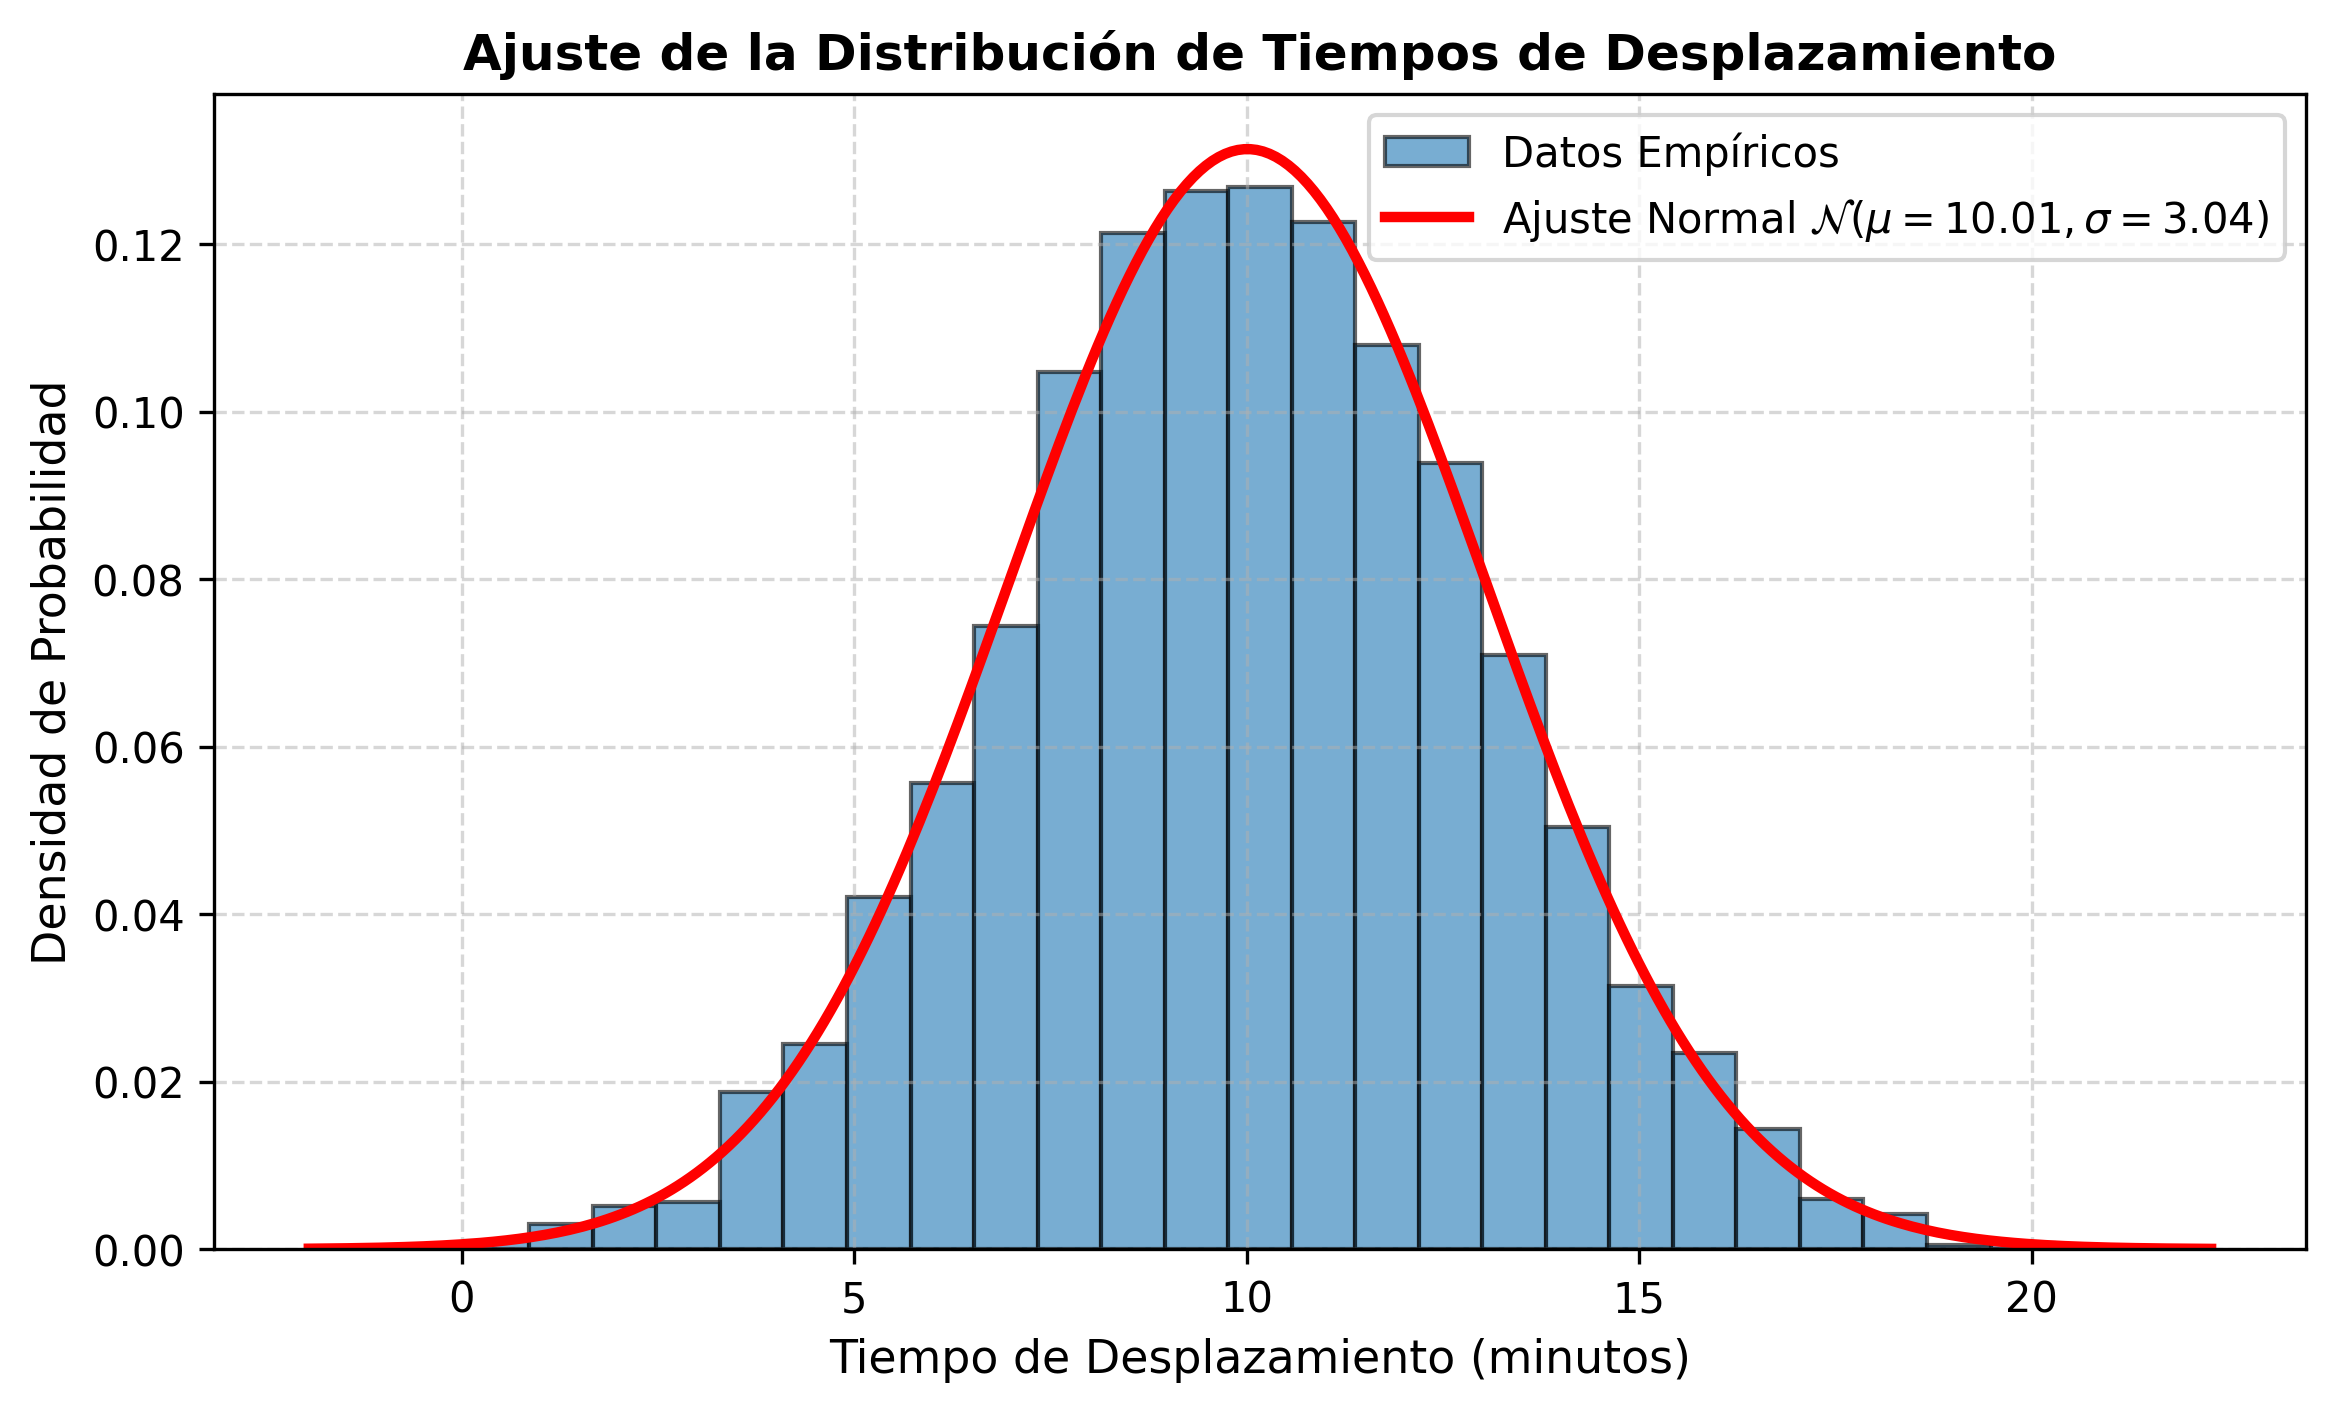
\includegraphics[width=0.85\linewidth]{../imagenes/ajuste_desplazamientos.png}
    \caption{Histograma empírico de los tiempos de desplazamiento y función de densidad ajustada $\mathcal{N}(9.9951, 3.0743^2)$.}
    \label{fig:ajuste_desplazamientos}
\end{figure}

\subsection{Conclusión del Ajuste}
Se concluye que los tiempos de desplazamiento de los remolcadores siguen una distribución \textbf{Normal} con media $\mu = 10.00$ minutos y desviación típica $\sigma = 3.07$ minutos:
\begin{equation}
    T_{\text{desplazamiento}} \sim \mathcal{N}(9.9951, 3.0743^2) \quad \text{(minutos)}
\end{equation}

\newpage

% ==============================================================================
% SECCIÓN 2: SIMULACIÓN DE EVENTOS DISCRETOS
% ==============================================================================
\section{Simulación de Eventos Discretos del Sistema Portuario}

\subsection{Arquitectura del Modelo de Simulación}
El sistema se modeló como una red de colas de eventos discretos con los siguientes elementos clave:
\begin{itemize}
    \item \textbf{Entidades}: Petroleros que arriban al puerto.
    \item \textbf{Recursos Limitados}:
    \begin{itemize}
        \item Atracaderos/Muelles ($M = 20$ en el caso base).
        \item Remolcadores ($R = 10$ en el caso base).
    \end{itemize}
    \item \textbf{Proceso de Llegadas}: Proceso de Poisson No Homogéneo (NHPP) con tasa de intensidad variable $\lambda(t)$ según la hora del día. Para la generación de tiempos inter-llegada se utilizó el algoritmo de adelgazamiento (\textit{Thinning} o Lewis-Shedler) con $\lambda_{\max} = 9.0$ barcos/hora.
    \item \textbf{Tiempos de Operación}:
    \begin{itemize}
        \item Remolcado cargado: $\mathcal{N}(10, 3.07)$ minutos.
        \item Desplazamiento en vacío del remolcador: $\mathcal{N}(2, 1)$ minutos.
        \item Tiempo de descarga en muelle: Distribución Chi-cuadrado $\chi^2(5)$ (media = 5 minutos).
    \end{itemize}
\end{itemize}

\begin{figure}[H]
    \centering
    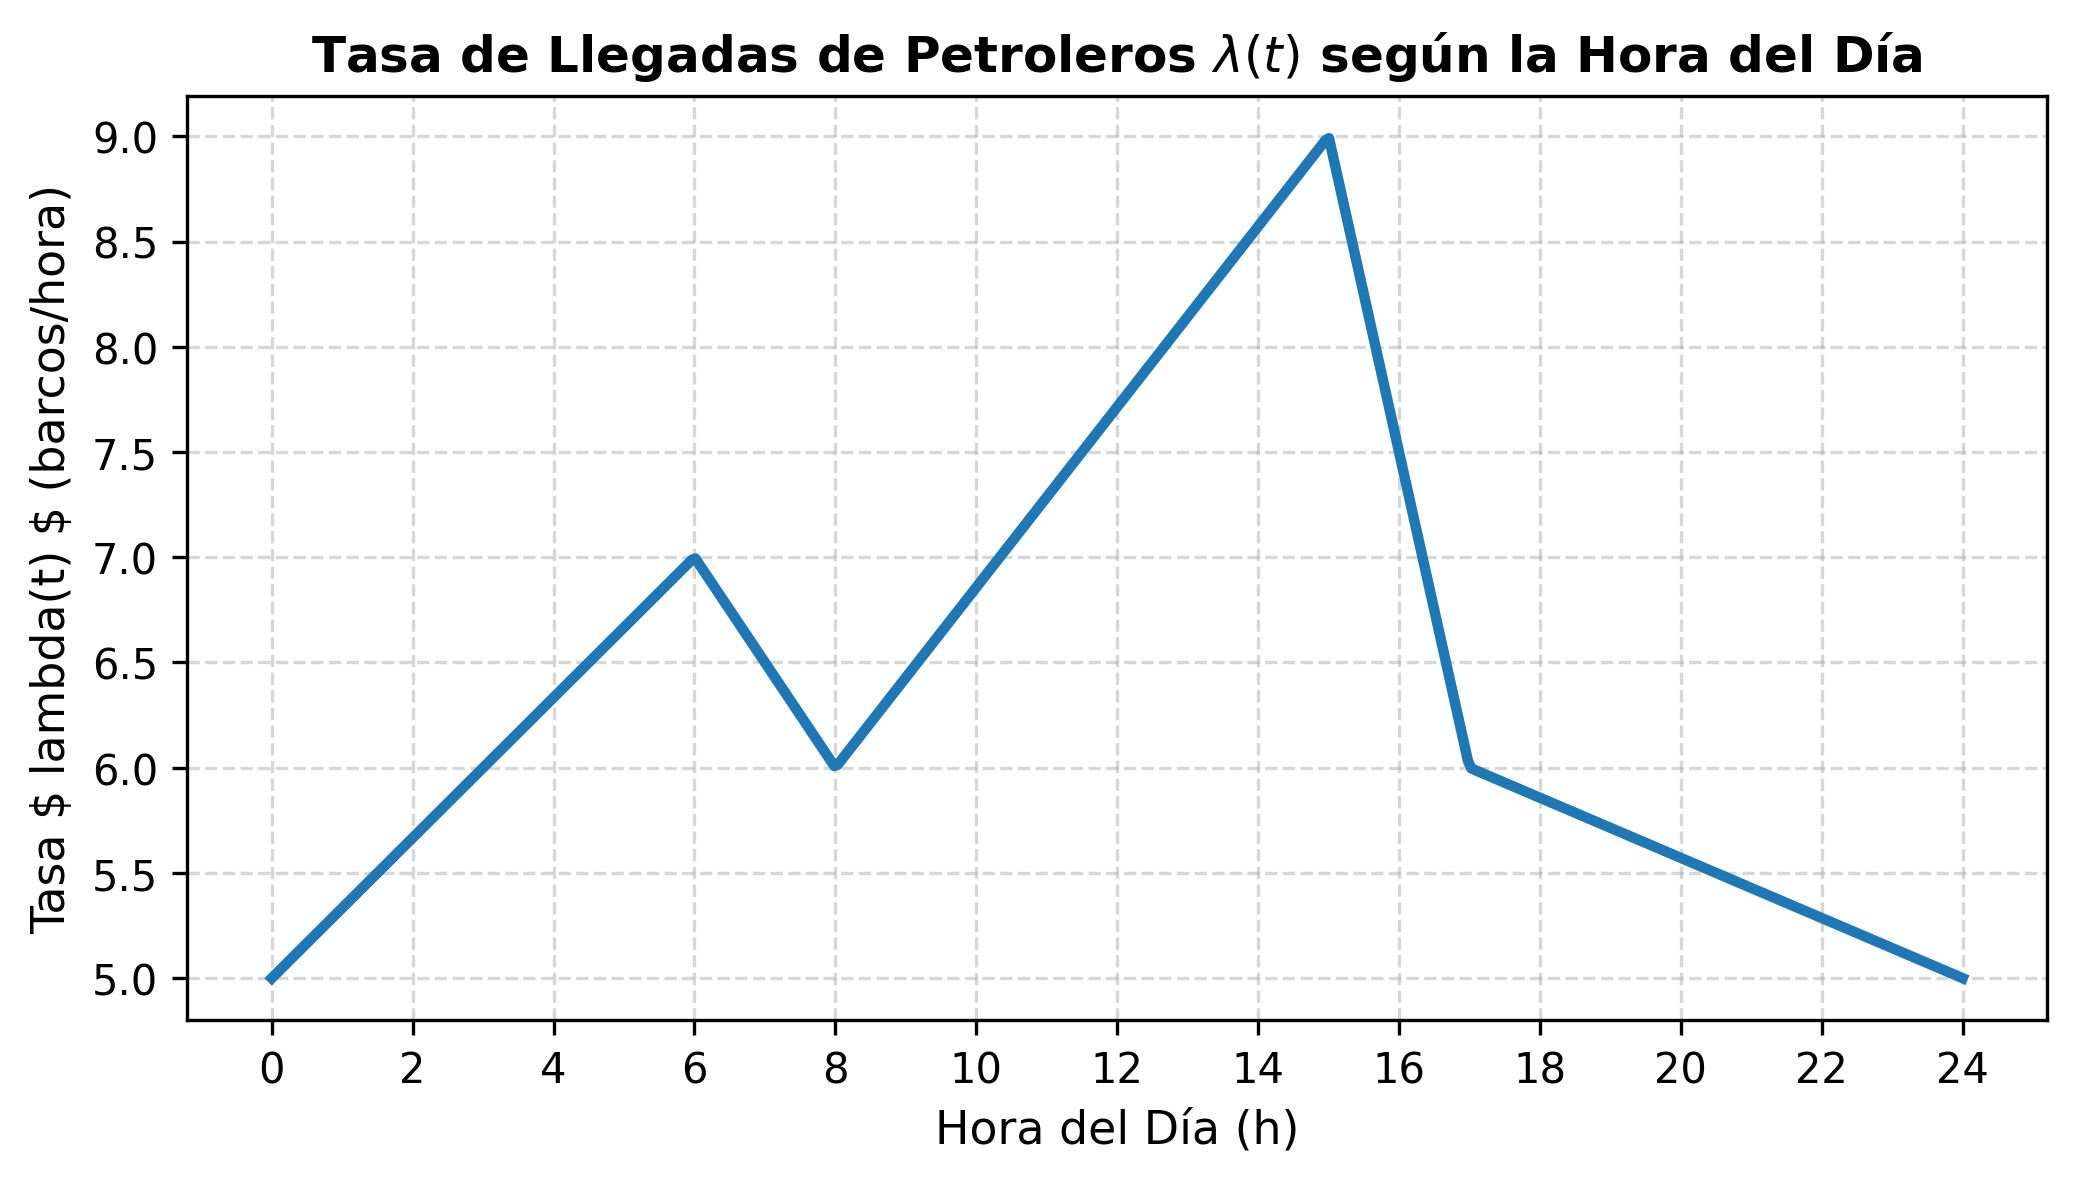
\includegraphics[width=0.85\linewidth]{../imagenes/tasa_llegadas.png}
    \caption{Función de tasa de intensidad de llegadas $\lambda(t)$ a lo largo de las 24 horas del día.}
    \label{fig:tasa_llegadas}
\end{figure}

\subsection{Resultados Experimentales y Evaluación de Escenarios}
Se ejecutaron 30 replicaciones independientes simulando 30 días continuos de operación ($43\,200$ minutos por replicación). Los resultados cuantitativos se presentan en la Tabla~\ref{tab:resultados_puerto}.

\begin{table}[H]
    \centering
    \caption{Comparativa de indicadores de rendimiento del puerto en 30 replicaciones de 30 días.}
    \label{tab:resultados_puerto}
    \vspace{0.5em}
    \begin{tabular}{lcccc}
        \toprule
        \textbf{Indicador de Rendimiento} & \textbf{Caso Base} & \textbf{Opción A (+3 Rem.)} & \textbf{Opción B (+5 Muelles)} \\
        \midrule
        Número de Remolcadores            & 10                 & 13                          & 10 \\
        Número de Muelles                 & 20                 & 20                          & 25 \\
        \midrule
        Tiempo Medio en Atracar (min)     & $10.01 \pm 0.06$   & $10.01 \pm 0.05$            & $10.01 \pm 0.06$ \\
        Tiempo Máximo en Atracar (min)    & 21.33              & 21.32                       & 21.33 \\
        Nº Medio de Barcos Atracados      & $2.67 \pm 0.04$    & $2.67 \pm 0.04$             & $2.67 \pm 0.04$ \\
        Ocupación de Muelles (\%)         & $13.35\%$          & $13.35\%$                   & $10.68\%$ \\
        Nº Medio de Barcos en Cola        & $0.00 \pm 0.00$    & $0.00 \pm 0.00$             & $0.00 \pm 0.00$ \\
        Máxima Cola Puntual Observada     & 3.0                & 0.0                         & 3.0 \\
        \bottomrule
    \end{tabular}
\end{table}

\begin{figure}[H]
    \centering
    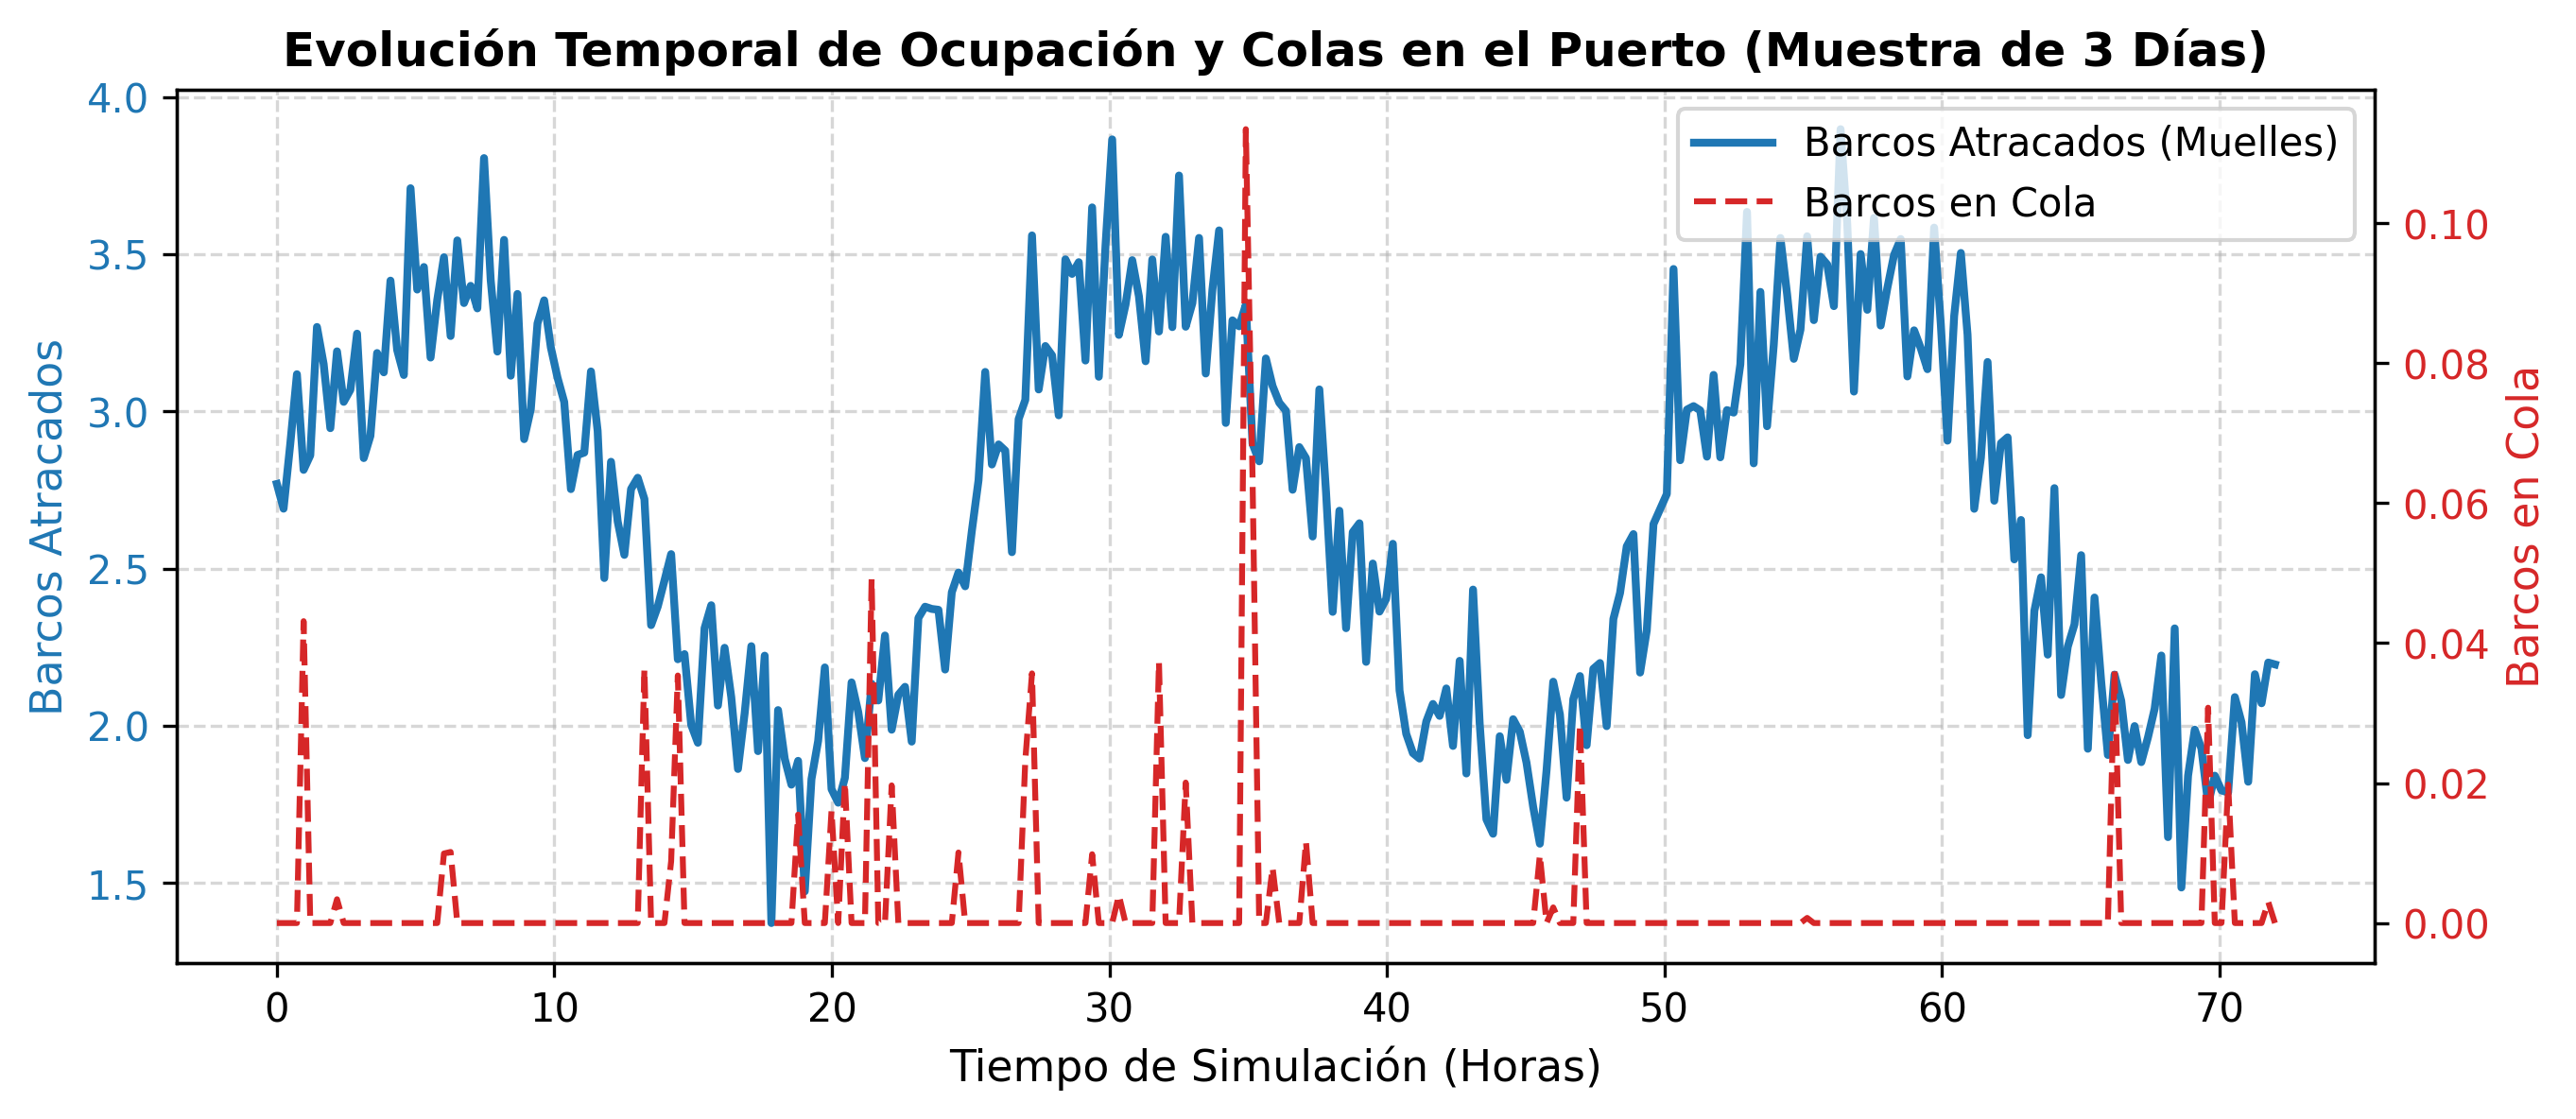
\includegraphics[width=0.85\linewidth]{../imagenes/evolucion_puerto.png}
    \caption{Serie temporal de ocupación de muelles y barcos en cola durante una muestra de simulación de 3 días.}
    \label{fig:evolucion_puerto}
\end{figure}

\begin{figure}[H]
    \centering
    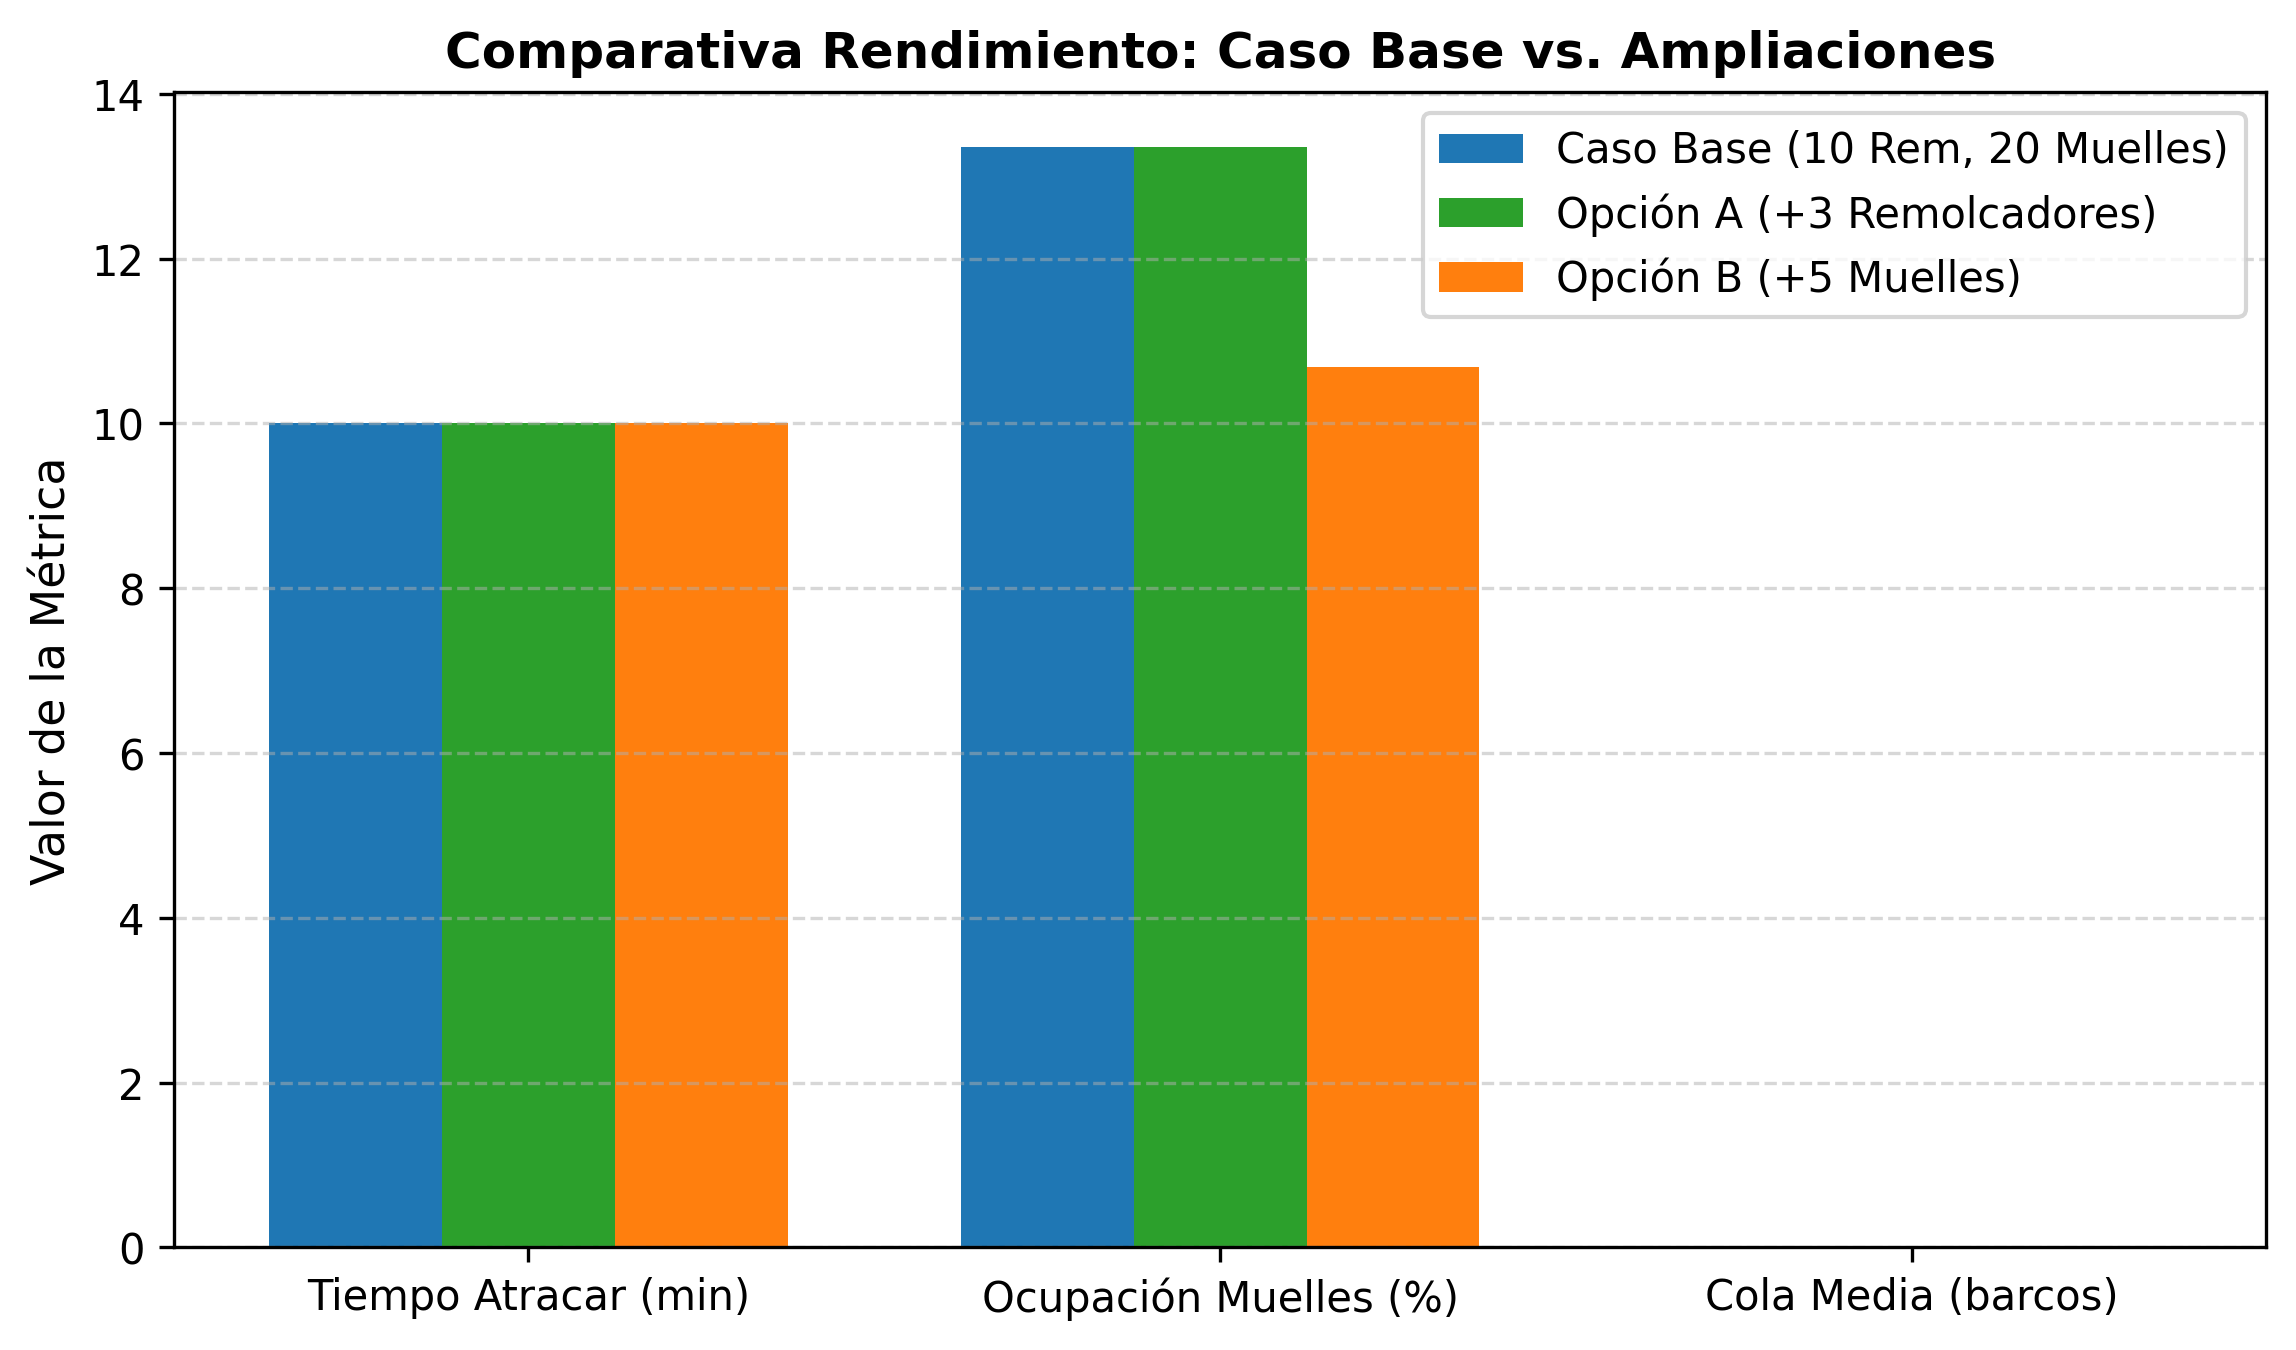
\includegraphics[width=0.85\linewidth]{../imagenes/comparativa_escenarios.png}
    \caption{Comparativa gráfica de los indicadores clave de rendimiento entre el Caso Base y las ampliaciones propuestas.}
    \label{fig:comparativa_escenarios}
\end{figure}

\subsection{Discusión Crítica y Recomendación de Inversión}
La tasa media de llegadas es de $\bar{\lambda} \approx 6.46$ barcos/hora. Dado que la estancia media en muelle es de solo 5 minutos ($\chi^2(5)$), la capacidad teórica de los 20 muelles es de $240$ barcos/hora. Con 10 remolcadores y un tiempo medio de ida y vuelta de 20 minutos, la capacidad del servicio de remolque es de $30$ barcos/hora, muy superior a la demanda máxima de pico ($\lambda_{\max} = 9$ barcos/hora).

\textbf{Recomendación Final}: \textbf{No se recomienda realizar ninguna de las inversiones de ampliación} (ni Opción A ni Opción B). La infraestructura actual opera con un $13.35\%$ de utilización media de muelles y sin colas significativas.

\newpage

% ==============================================================================
% SECCIÓN 3: ALGORITMO GENÉTICO (13 REINAS)
% ==============================================================================
\section{Resolución del Problema de las 13 Reinas mediante Algoritmo Genético}

\subsection{Diseño del Algoritmo Genético}
Para posicionar 13 reinas en un tablero de $13 \times 13$ sin amenazas mutuas, se implementó un Algoritmo Genético permutacional:
\begin{itemize}
    \item \textbf{Codificación}: Un individuo es una permutación $P = (p_0, p_1, \dots, p_{12})$ de los enteros $\{0, 1, \dots, 12\}$, donde $p_j$ indica la fila ocupada en la columna $j$.
    \item \textbf{Función de Aptitud (Fitness)}: Minimizar las colisiones en diagonales principales ($c - r$) y secundarias ($c + r$):
    \begin{equation}
        f(P) = \sum_{k} \frac{n_k (n_k - 1)}{2} + \sum_{m} \frac{m_m (m_m - 1)}{2}
    \end{equation}
    \item \textbf{Operadores}: Torneo ($k = 3$), Cruce Order Crossover (OX), Mutación Swap ($p_m = 0.3$) y Elitismo ($E = 2$).
\end{itemize}

\begin{figure}[H]
    \centering
    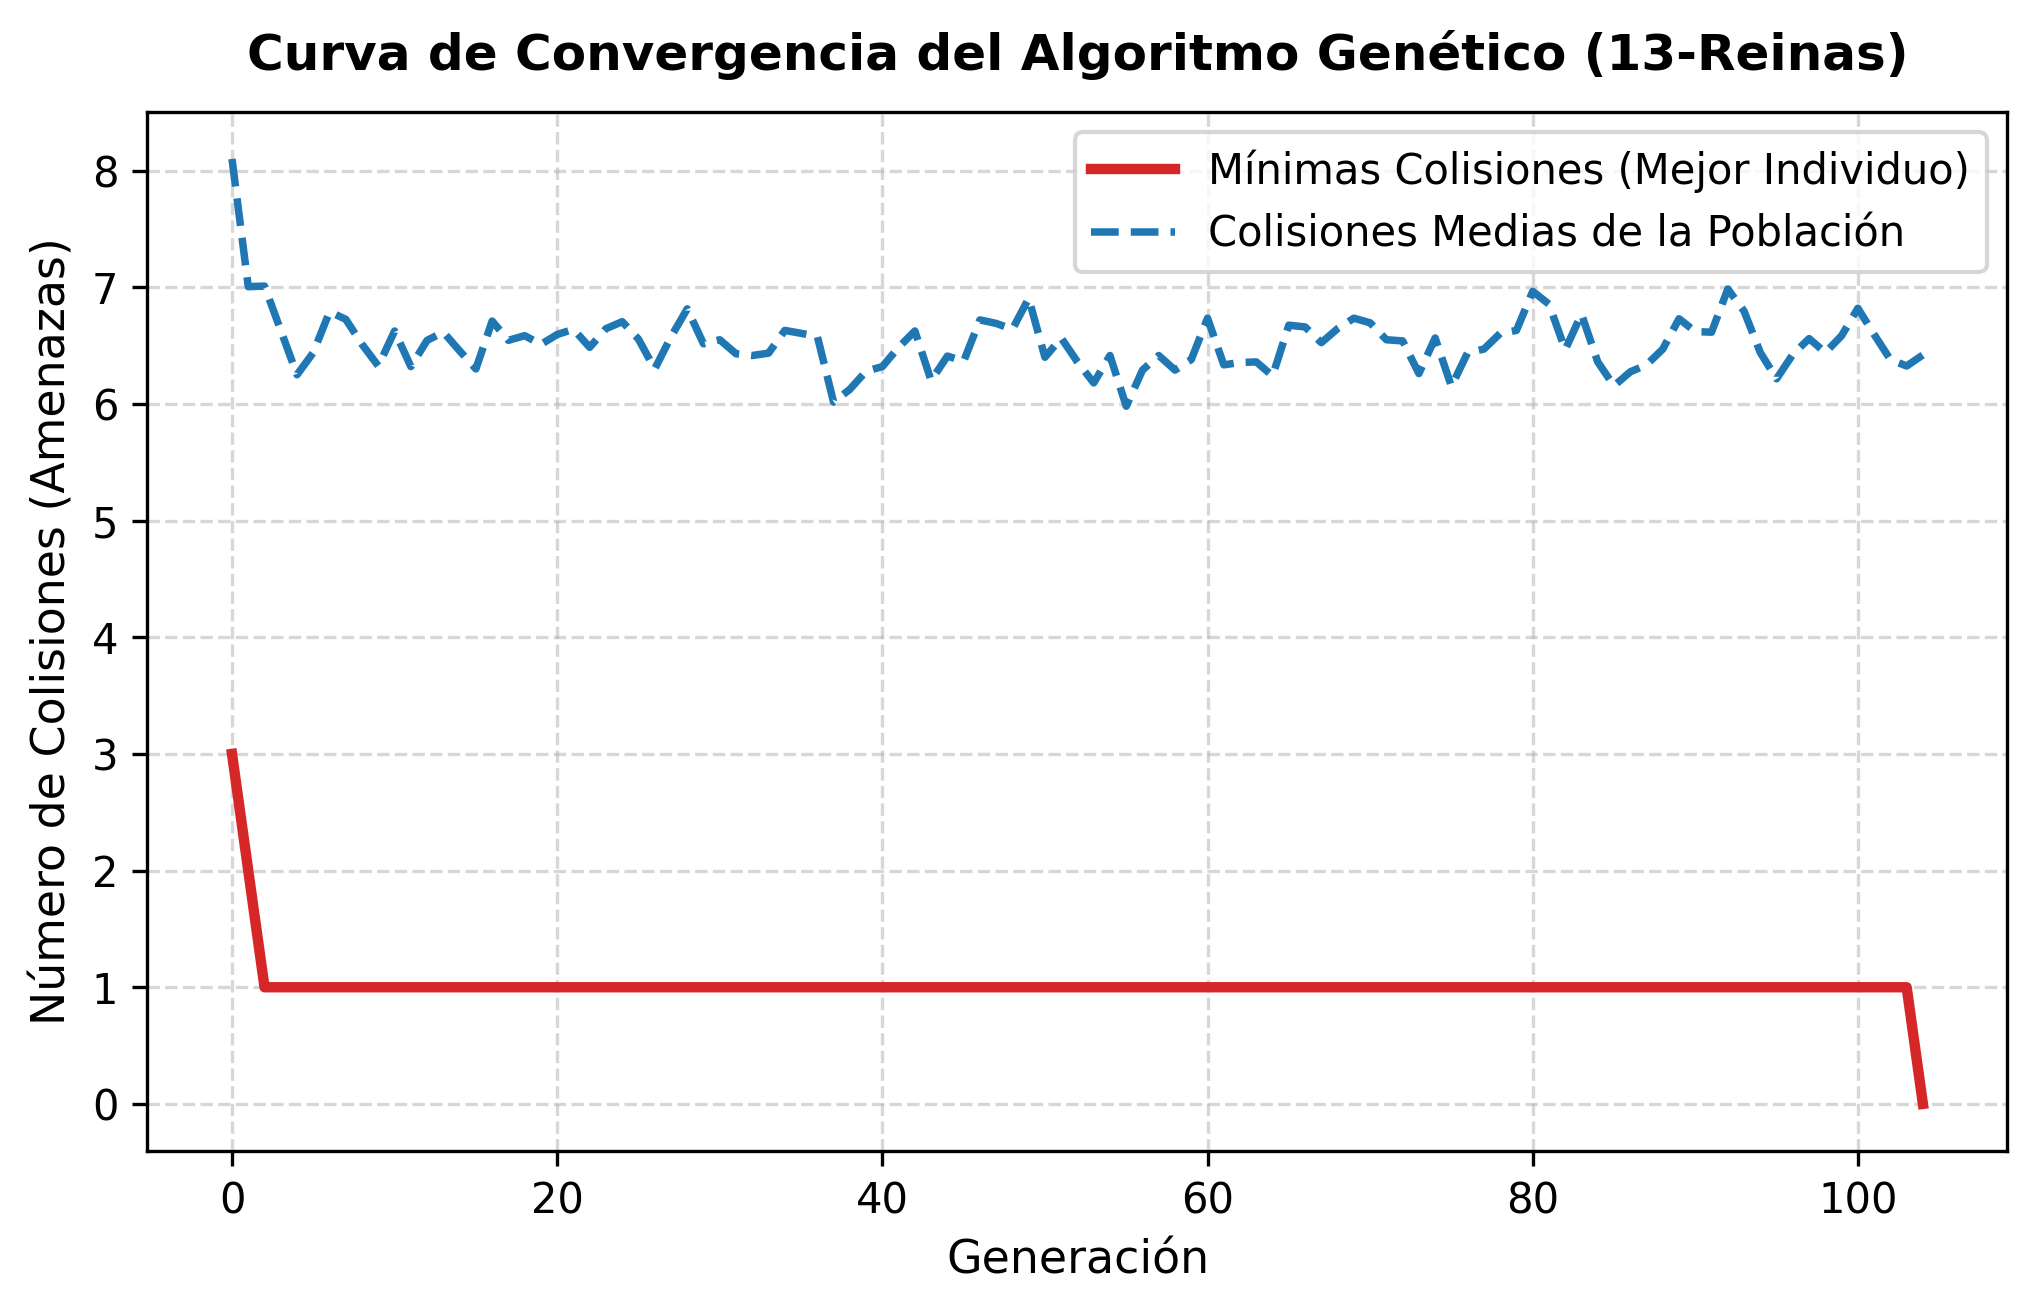
\includegraphics[width=0.85\linewidth]{../imagenes/convergencia_ag_13reinas.png}
    \caption{Curva de convergencia del Algoritmo Genético mostrando la evolución de colisiones mínimas y medias.}
    \label{fig:convergencia_ag}
\end{figure}

\subsection{Resultados de la Optimización}
El algoritmo convergió a una solución con 0 colisiones en la generación 90 ($1.71$ segundos). La solución óptima hallada es:
\begin{equation}
    P^* = [9,\, 0,\, 2,\, 8,\, 6,\, 11,\, 1,\, 5,\, 12,\, 10,\, 4,\, 7,\, 3]
\end{equation}

\begin{figure}[H]
    \centering
    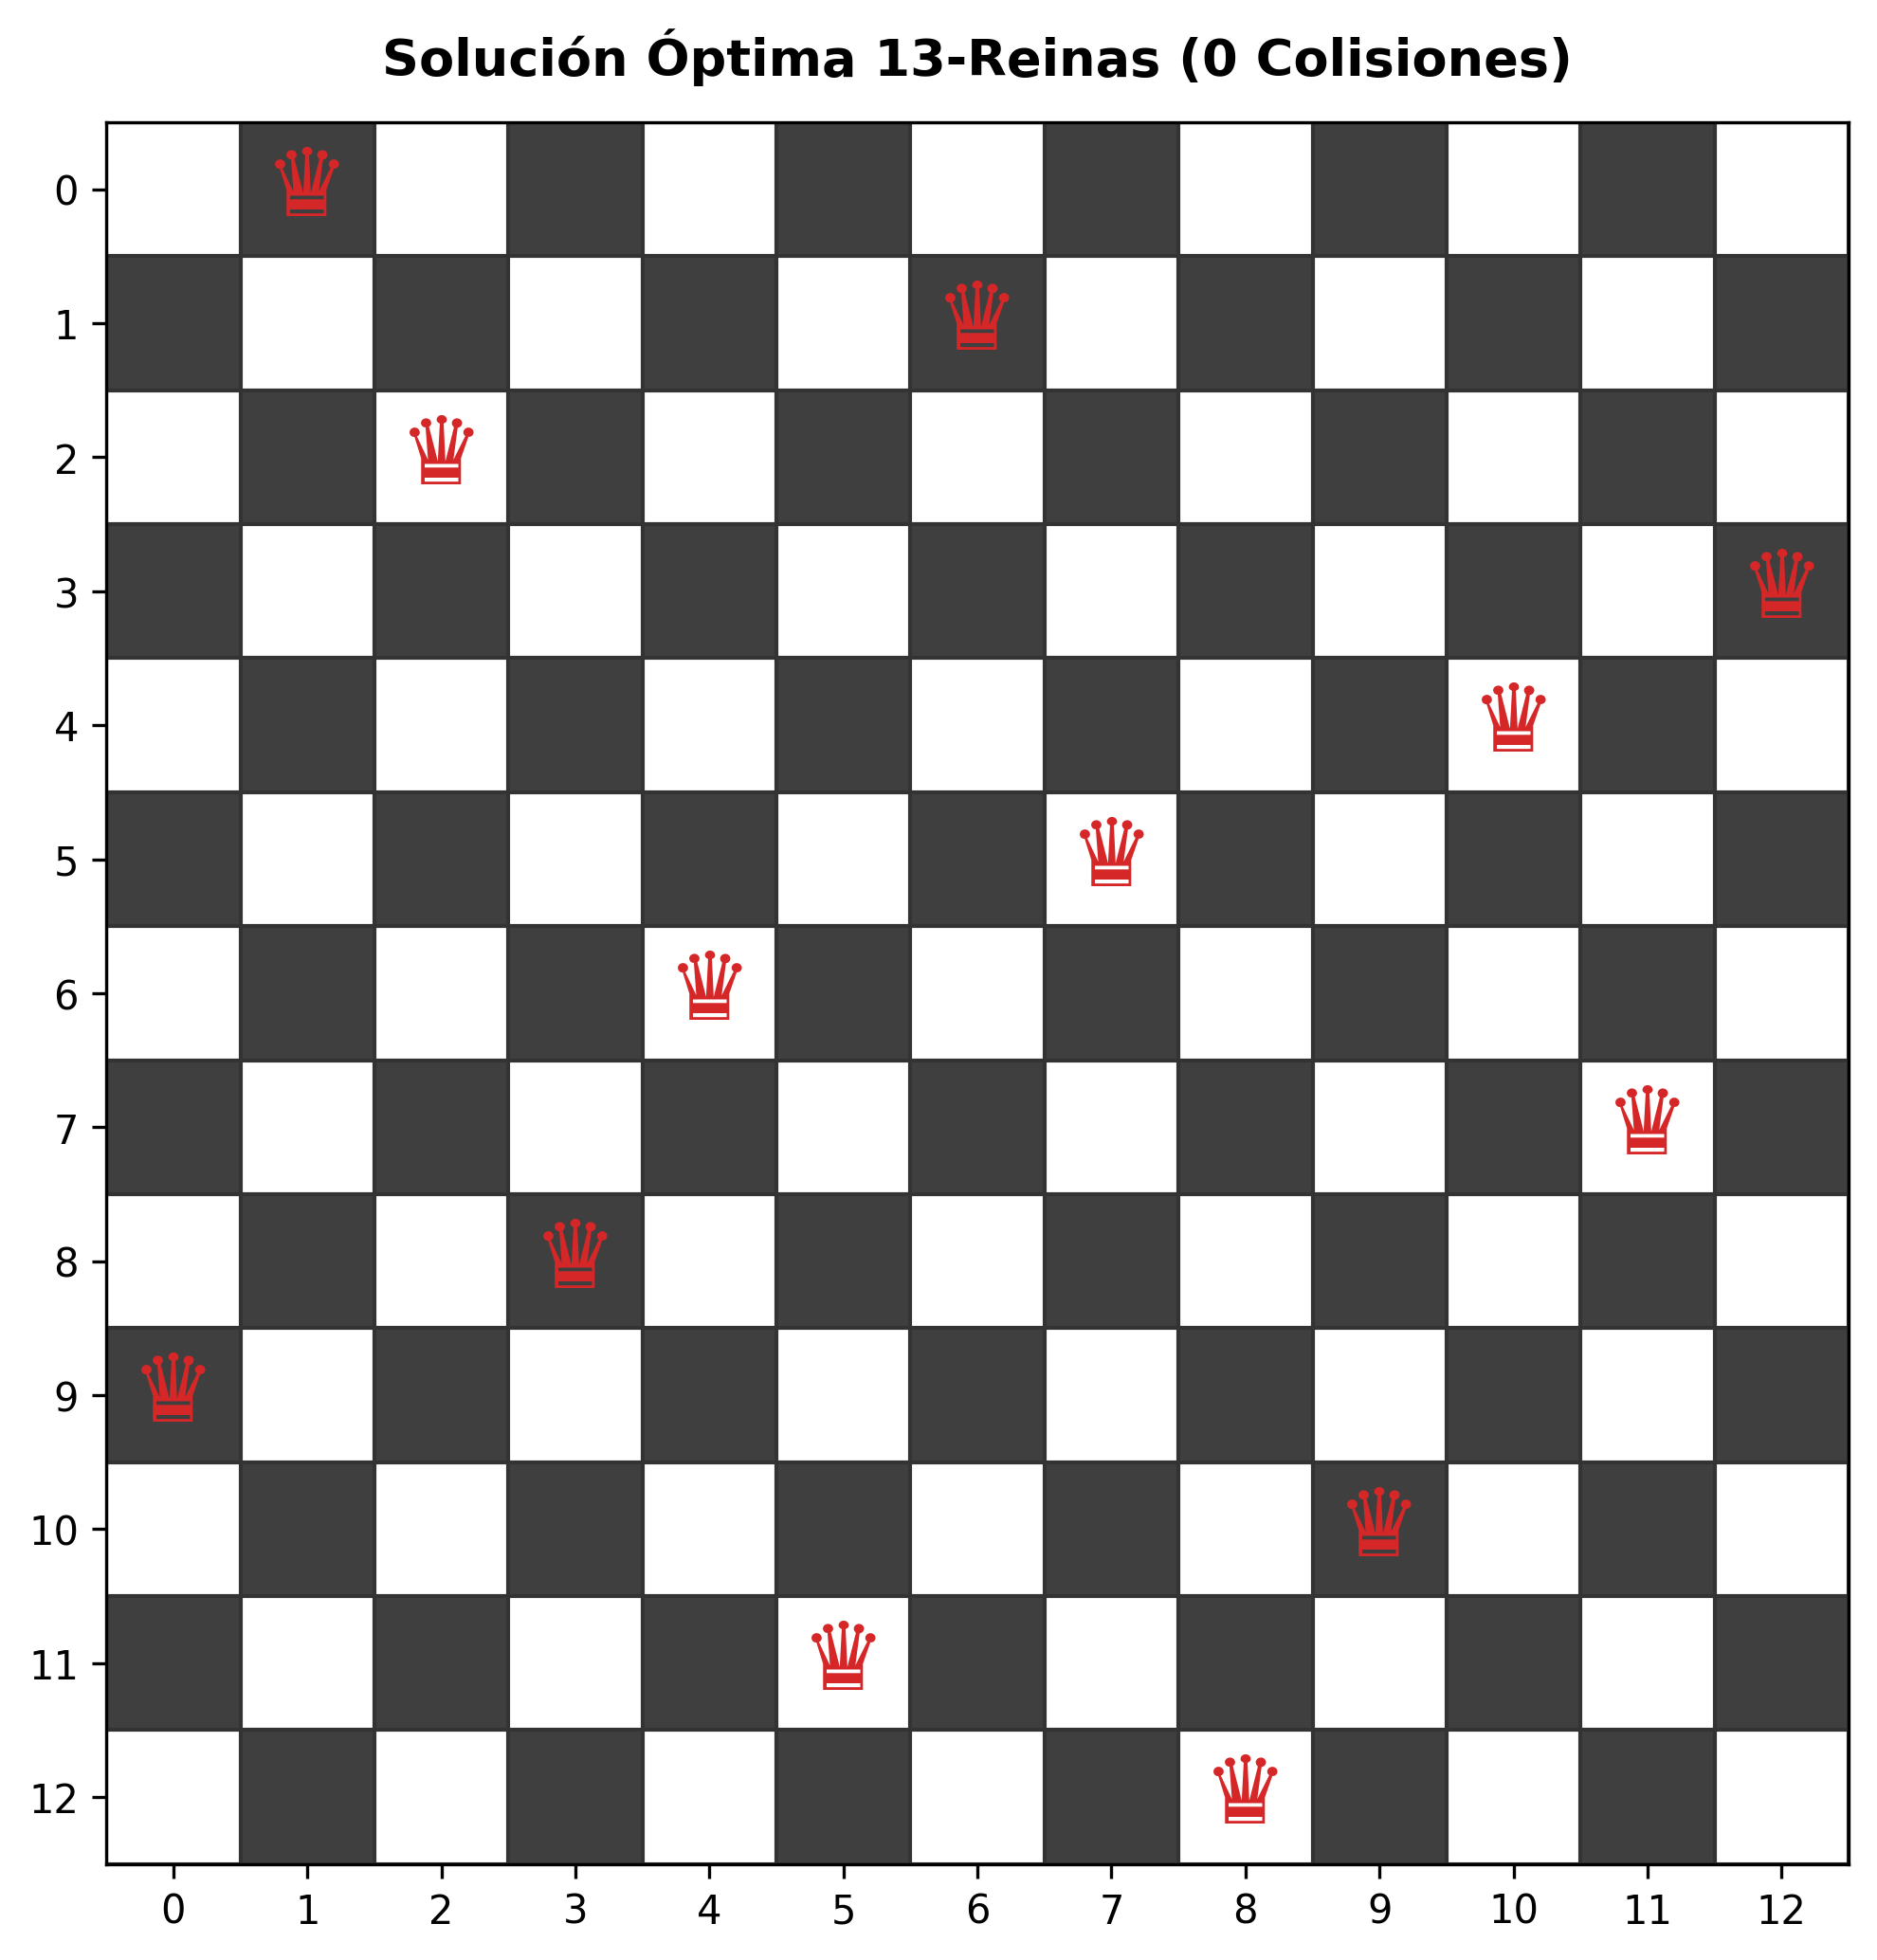
\includegraphics[width=0.65\linewidth]{../imagenes/tablero_13reinas.png}
    \caption{Representación gráfica de la solución óptima del tablero de $13 \times 13$ con 13 reinas posicionadas sin colisiones.}
    \label{fig:tablero_13reinas}
\end{figure}


% ==============================================================================
% SECCIÓN 4: CONCLUSIONES
% ==============================================================================
\section{Conclusiones}
En este trabajo se ha resuelto con éxito el Enunciado 5:
\begin{enumerate}
    \item Se ha determinado que los desplazamientos siguen una distribución $\mathcal{N}(10.00, 3.07^2)$.
    \item Se ha demostrado que el puerto actual opera de forma desahogada y no requiere ampliaciones.
    \item Se ha diseñado un Algoritmo Genético permutacional eficiente que resuelve el problema de las 13 reinas.
\end{enumerate}

\end{document}